\documentclass[12pt,letterpaper]{article}
\usepackage{fullpage}
\usepackage[top=2cm, bottom=4.5cm, left=2.5cm, right=2.5cm]{geometry}
\usepackage{amsmath,amsthm,amsfonts,amssymb,amscd}
\usepackage{lastpage}
\usepackage{enumerate}
\usepackage{amsmath}
\usepackage{algorithm}
\usepackage[noend]{algpseudocode}
\usepackage{fancyhdr}
\usepackage{mathrsfs}
\usepackage{xcolor}
\usepackage{graphicx}
\usepackage{listings}
\usepackage{hyperref}
\usepackage{algpseudocode}

\makeatletter
\def\BState{\State\hskip-\ALG@thistlm}
\makeatother

\hypersetup{%
  colorlinks=true,
  linkcolor=blue,
  linkbordercolor={0 0 1}
}
 
\renewcommand\lstlistingname{Algorithm}
\renewcommand\lstlistlistingname{Algorithms}
\def\lstlistingautorefname{Alg.}

\lstdefinestyle{C++}{
    language        = C++,
    frame           = lines, 
    basicstyle      = \footnotesize,
    keywordstyle    = \color{blue},
    stringstyle     = \color{green},
    commentstyle    = \color{red}\ttfamily
}

\setlength{\parindent}{0.0in}
\setlength{\parskip}{0.05in}

% Edit these as appropriate
\newcommand\course{COT 5405}
\newcommand\hwnumber{1}                  % <-- homework number
\newcommand\name{Saksham Bathla}
\newcommand\NetIDa{UFID : 8296-7553}           % <-- NetID of person #1


\pagestyle{fancyplain}
\headheight 35pt
\lhead{\NetIDa \\ \name}
\chead{\textbf{\Large Homework \hwnumber}}
\rhead{\course \\ \today}
\lfoot{}
\cfoot{}
\rfoot{\small\thepage}
\headsep 1.5em

\begin{document}

\section*{Problem 1 : Cycle Detection}
Given an undirected graph G (V,E), we have to identify a cycle in the graph.  \hfill \break
\textbf{Algorithm:}
\begin{algorithm}
    \caption{Cycle Detection Using DFS}\label{euclid}
    \begin{algorithmic}[1]
    \Procedure{DetectCycle(graph)}{}
    \For {$vertex \textit{ in } $graph.vertexSet}
    \If {$\textit{visited[vertex]} \gets \textit{true}$}
    \State $\textit{continue}$
    \EndIf
    \If {$DetectCycleUtil(vertex,null,visited,graph)$} 
    \Return true
    \EndIf
    \EndFor
    \Return $\textit{false}$
    \EndProcedure
    \Procedure{DetectCycleUtil(source, parent, visited, graph)}{}
    \State $\textit{visited[vertex]}\gets \textit{true}$
    \State $adjacentVertices \gets graph.adjacencyList[vertex]$
    \For {$adjVertex \textit{ in } $adjacentVertices}
    \If {$\textit{visited[adjVertex]}\gets \textit{true}$}
    \Return $\textit{true}$
    \EndIf
    \If {$DetectCycleUtil(adjVertex,vertex,visited,graph)$}
    \Return true
    \EndIf
    \EndFor
    \Return false
    \EndProcedure
    \end{algorithmic}
\end{algorithm}

\begin{enumerate}


\item 
\textbf{Proof of Correctness:}
  
  G = (V,E) \newline
Let us assume that there exists a cycle in the graph after the completion of the algorithm having not found any cycle.\newline
\implies{\exists \textit{ a path P in G s.t. P starts with a vertex v and ends with the same vertex}}\newline
\textit {But as we use recursion to traverse all possible paths starting from v and stop on reaching v again}\newline 
\therefore {$\textit{the path P would have been found in the running of the algorithm}$}\newline 
\implies {$\textit{Our assumption was incorrect}$}\newline
\textit{Hence proved}
  
  
\newpage
\item
\textbf{Proof of Runtime:}
If there exists a cycle, then worst case will be that all nodes are a part of the cycle. In this case, the DetectCycle procedure would visit each vertex once and each edge only twice since we are keeping a track of all nodes visited previously. Hence, the complexity would be O(V+E). \newline
In case of no cycle, then recursion would still visit each vertex once. Hence, the complexity would still be O(V+E).
\newline
\end{enumerate}

\textbf{Figure 1} and \textbf{Figure 2} show the plot of time taken in case of worst case as well as random inputs.
\begin{figure}[!h]
\centering
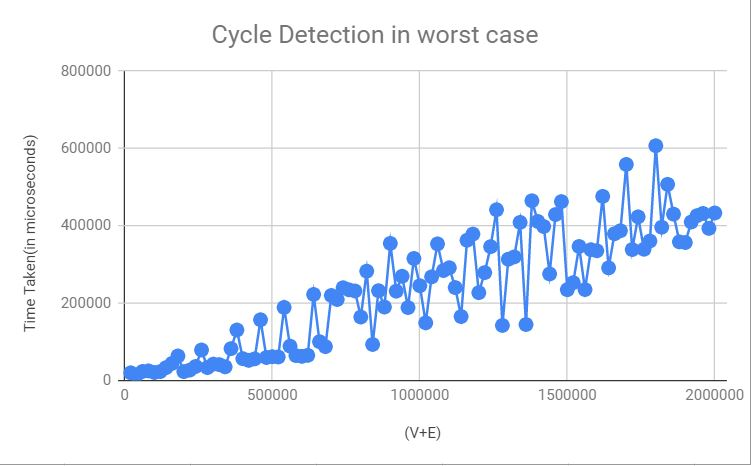
\includegraphics[width=0.5\linewidth]{cycle_worst_case.JPG}
\caption{running time as a function of size in case of worst case input}
\end{figure}
\begin{figure}[!h]
\centering
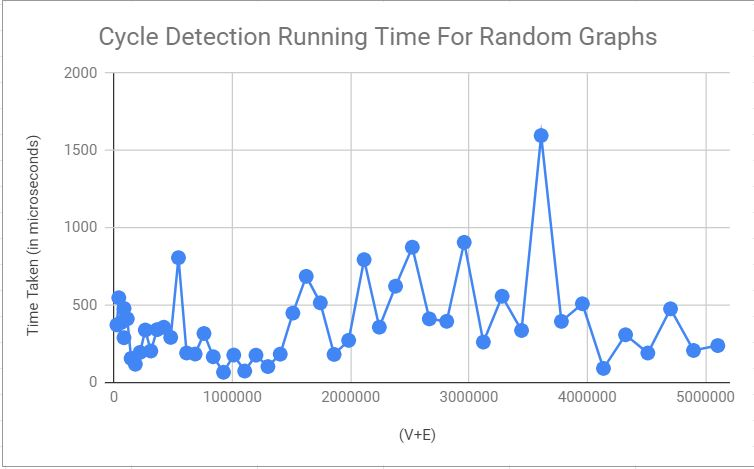
\includegraphics[width=0.5\linewidth]{rand_cyc.JPG}
\caption{running time as a function of size in case of random input}
\end{figure}
\newpage

\section*{Problem 2 : Minimum Spanning Tree for Sparse Graphs}
For a sparse graph G(V,E), with maximum number of edges = number of vertices + 8, we have to find the MST of the graph \hfill \break
\begin{algorithm}
    \caption{MST using Reverse Delete Algorithm}\label{euclid}
    \begin{algorithmic}[1]
    
    \Procedure{getMst(graph)}{}
    \State $edgeSet \gets sort(graph.edgeSet) $
    \State $mstWeight \gets 0$
    \State $i \gets numEdges-1$
    \While{$i \ge 0$}{
    \State $edgeSet' \gets removeEdge(edgeSet[i])$.
    \If {$ isConnected(G,edgeSet') \neq true$}
    \State $mstWeight \gets WeightOf(edgeSet[i])$
    \State $edgeSet' \gets add Edge(edgeSet[i])$.
    \EndIf
    \State $i \gets i-1$.
    \EndWhile}
    \Return $mstWeight$
    \EndProcedure
    \end{algorithmic}
\end{algorithm}
\begin{enumerate}

\linebreak
\textbf{Proof of Correctness :}\newline

\item
\textbf{Proof That the final graph is a spanning tree:}

We reverse sort the edges of the connected Graph G(V,E) by weight and start removing edges from G such that G’(V,E’) = G(V,E) – max(e). Then we check using isConnected(), if the graph remains connected. If the graph gets disconnected, we add the edge back. Hence, after each operation the graph results in a connected graph. We keep repeating this operation until no cycles are found. Hence, this results in a spanning tree. \hfill \hfill
\newpage

\item
\textbf{Proof of Minimum Weight:}

We begin with sorting the edges such that
w_{e1} > w_{e2} > w_{e3} …… > w_{n}

During each iteration we remove the maximum weight edge if it doesn't lead to disconnection.

If we assume that the resulting graph is not the minimum spanning tree, this implies that there must be an edge in the final graph with higher weight then one of the removed edges which could have been removed.

But, since we started with removing higher weights edge and checked the connectivity at each iteration, It means that the higher weight edge must have been removed first if it didn't lead to a disconnected graph.  

Hence, no edge exists in the graph that could be replaced with a lesser weight edge resulting in an MST. 

Hence proved.
\newline\newline
\textbf{Proof of Runtime:} O(E.log(E))\newline

In this implementation, we first sort the edgeSet, which happens in \texit{O(E.log(E))} time. Then, for each edge, we perform the find and union in our disjoint set of vertices (with union by rank and path compression) which gives a complexity of O(V) Since V ~ E, our Complexity becomes O(E.log(E)). 


\end{enumerate}
\begin{figure}[!h]
\centering
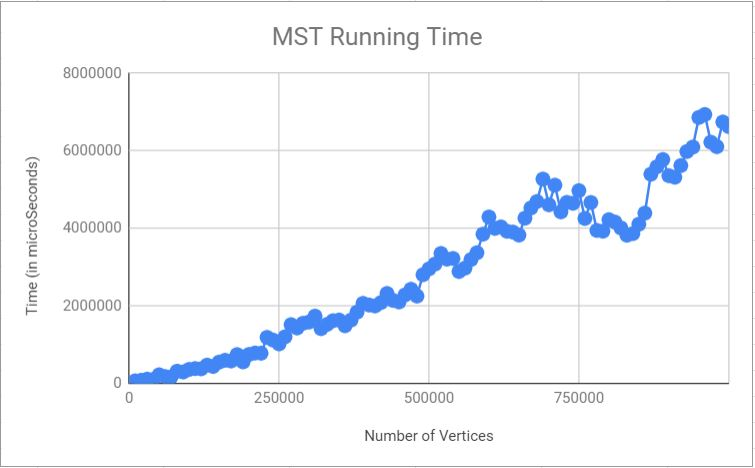
\includegraphics[width=0.5\linewidth]{mst.JPG}
\caption{running time as a function of size in case of random input}
\end{figure}

\newpage
\section*{Implementation}
\begin{enumerate}
\item\textbf{Running this code: }\newline\newline
\textbf{Problem 1 :} \newline
The graph generator generates a graph using Jgrapht library graph generation function. I have also generated a worst case graph generation function where we create a random tree with no cycles, so as to test the algorithm for the worst case inputs\newline

Code File: CycleFinder.java \newline\newline
To run: java -cp lib/jgrapht-core-1.5.1.jar CycleFinder.java\newline\newline

\textbf{Problem 2:} 
Here we start by generating a random tree by making randomly selecting children for each node and avoiding any back edges. After doing so, we add a random number of edges (between 0 and 9) in the graph to simulate the sparse graph\newline

Code file : Mst.Java \newline\newline
To run: java -cp lib/jgrapht-core-1.5.1.jar Mst.java\newline\newline

\item\textbf{Testing and evaluation: }\newline\newline
\textbf{Problem 1:} \newline\newline
1). I generated different acyclic graph of various sizes too test the correctness and worst case runtime of the algorithm. I checked the correctness of the algorithm against the jgrapht library functions available to find cycles and to check for acyclicity\newline\newline
2). I generated various random graphs using the Jgrapht random graph generator and tested the time taken as well as correctness against the library functions available in jgrapht. For testing correctness, I also generated some small sized hard-coded graphs to check the corretness of the algorithm\newpage
\textbf{Problem 2:} \newline\newline
1). Here we started by generating a random tree by making randomly selecting children for each node and avoiding any back edges. then I added random edges to this tree to produce the required sparse graph. To test for correctness, I checked it against the library function for MST in jgrapht and ran it on vertex sizes upto 1000000 to plot the time complexity. 
\newline\newline
\end{enumerate}
\end{document}
